\documentclass[a4paper,12pt]{scrartcl} 
\usepackage[utf8]{inputenc}
\usepackage{graphicx}
\usepackage[numbib]{tocbibind}
\usepackage{gensymb}
\usepackage{pgfplots}
\usepackage{tikz}
\usepackage{hyperref}
\usepackage{microtype}
\usepackage{lmodern}
\usepackage[T1]{fontenc}
\usepackage{geometry}
\usepackage{float}
\usetikzlibrary{positioning,shapes,shadows,arrows,chains}
\usepackage{mathtools,amsfonts,amssymb}
\usepackage{graphicx}
\usepackage{minted}

\tikzset{%
	cell/.style={%
		rectangle split,
		rectangle split parts=4,
		rectangle split horizontal,
		rectangle split part fill={lightgray!30},
		rectangle split empty part width=0.1cm,
		draw
	}
}

\begin{document}

\begin{titlepage}
    \author{Sven-Hendrik Haase}
    \title{Alignment sin C}
    \subtitle{Seminar ``Effiziente Programmierung in C''}
    \date{2014-01-09}
    \maketitle
    \thispagestyle{empty}
\end{titlepage}

\tableofcontents

\newpage

\section{Introduction}
Working with memory is currently the most time consuming task in modern processors. As such, great
care has to be taken so that inefficiencies can be kept at a minimum. This document exists to
describe how memory addressing works in a modern processor and how data structures are aligned for
maximum performance during access.

\subsection{Memory Addressing}
\begin{itemize}
    \item Computers address memory in word-sized chunks
    \item A \textbf{word} is a computer's natural unit for data
    \item Word size is defined by architecture
    \item Usual word sizes: 4 byte on 32-bit, 8 byte on 64-bit
    \item This means we can only address data at memory locations that are
          multiples of 4 or 8 respectively (strictly speaking)
    \item Many processors allow access of arbitrary memory locations while some fail
        horribly
\end{itemize}

\begin{itemize}
    \item Modern processors can load word-sized (4 byte) and long word-sized (8 byte) memory
        locations equally well
    \item Find out word-sizes:
    \begin{itemize}
        \item \verb|getconf WORD_BIT| (32 for me)
        \item \verb|getconf LONG_BIT| (64 for me)
    \end{itemize}
\end{itemize}

\subsection{Alignment 101}
\begin{itemize}
    \item Assume a 32-bit architecture with a word size of 4 byte
        \begin{center}
            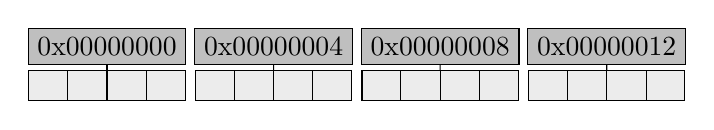
\begin{tikzpicture}[start chain, level distance=0.5cm, node distance=0.1cm, every on chain/.style={draw, fill=lightgray, minimum width=2cm}]
                \node [on chain] {0x00000000} child {node [cell] {}};
                \node [on chain] {0x00000004} child {node [cell] {}};
                \node [on chain] {0x00000008} child {node [cell] {}};
                \node [on chain] {0x00000012} child {node [cell] {}};
            \end{tikzpicture}
        \end{center}
    \item Let's save a 4 byte \textbf{int}
        \tikz[baseline=-0.5ex]{%
            \node[cell, rectangle split part fill={green!50},] {};} in our
        memory:
\end{itemize}
\begin{center}
    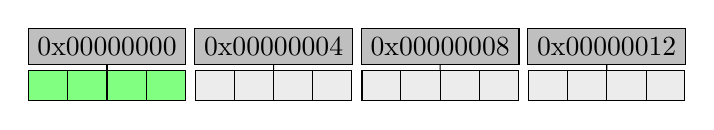
\begin{tikzpicture}[start chain, level distance=0.5cm, node distance=0.1cm, every on chain/.style={draw, fill=lightgray, minimum width=2cm}]
        \node [on chain] {0x00000000} child {node [cell, rectangle split part fill={green!50},] {}};
        \node [on chain] {0x00000004} child {node [cell] {}};
        \node [on chain] {0x00000008} child {node [cell] {}};
        \node [on chain] {0x00000012} child {node [cell] {}};
    \end{tikzpicture}
\begin{itemize}
    \item Looks good!
\end{itemize}
\end{center}

\begin{itemize}
    \item Let's save a \textbf{char}
        \tikz[baseline=-0.5ex]{%
            \node[cell, rectangle split part fill={red!50,lightgray!30}] {};}, a \textbf{short}
        \tikz[baseline=-0.5ex]{%
            \node[cell, rectangle split part fill={blue!50,blue!50,lightgray!30}] {};} and an \textbf{int}
        \tikz[baseline=-0.5ex]{%
            \node[cell, rectangle split part fill={green!50},] {};} in our memory:
\end{itemize}
\begin{center}
    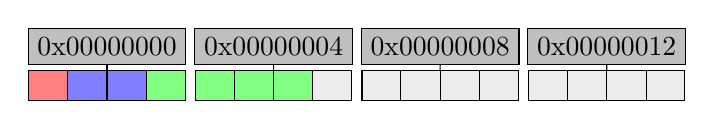
\begin{tikzpicture}[start chain, level distance=0.5cm, node distance=0.1cm, every on chain/.style={draw, fill=lightgray, minimum width=2cm}]
        \node [on chain] {0x00000000} child {node [cell, rectangle split part fill={red!50,blue!50,blue!50,green!50}] {}};
        \node [on chain] {0x00000004} child {node [cell, rectangle split part fill={green!50,green!50,green!50,lightgray!30}] {}};
        \node [on chain] {0x00000008} child {node [cell] {}};
        \node [on chain] {0x00000012} child {node [cell] {}};
    \end{tikzpicture}
\begin{itemize}
    \item Oh wait
    \item Needs two memory accesses and some arithmetic to fetch the \textbf{int}.
\end{itemize}
\end{center}

\begin{itemize}
    \item We need to be smarter about this!
    \item Padding \tikz[baseline=-0.5ex]{%
                    \node[cell, rectangle split part fill={darkgray,lightgray!30},] {};} to the
                    rescue
\end{itemize}
\begin{center}
    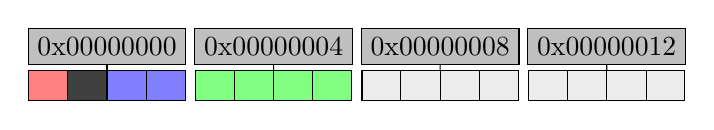
\begin{tikzpicture}[start chain, level distance=0.5cm, node distance=0.1cm, every on chain/.style={draw, fill=lightgray, minimum width=2cm}]
        \node [on chain] {0x00000000} child {node [cell, rectangle split part fill={red!50,darkgray,blue!50,blue!50}] {}};
        \node [on chain] {0x00000004} child {node [cell, rectangle split part fill={green!50}] {}};
        \node [on chain] {0x00000008} child {node [cell] {}};
        \node [on chain] {0x00000012} child {node [cell] {}};
    \end{tikzpicture}
\end{center}
\begin{itemize}
    \item Much better
    \item This is considered \textbf{naturally aligned}
\end{itemize}

\subsection{Consequences of Misalignment}
\begin{itemize}
    \item Different behavior depending on architecture
    \item Alignment fault errors on some platforms (RISC, ARM)
    \item Bad performance on others
    \item SSE requires proper alignment per specification (though this restriction is about to be removed)
\end{itemize}

\section{Data Structure Alignment}
\subsection{Example With Structs}
Consider this:
\begin{minted}{c}
struct Foo {
    char x; // 1 byte
    short y // 2 bytes
    int z; // 4 bytes
};
\end{minted}
\begin{itemize}
    \item The struct's naive size would be 1 byte + 2 bytes + 4 bytes = 7 bytes
    \item Of course, we know it's actually going to be 8 bytes due to padding
\end{itemize}

\begin{itemize}
    \item A struct is aligned to the largest type's alignment requirements
    \item This can yield some rather inefficient structures:
\end{itemize}
\begin{minted}{c}
struct Foo {
    char x; // 1 byte
    double y // 8 bytes
    char z; // 1 bytes
};
\end{minted}
\begin{itemize}
    \item The struct's naive size would be 1 byte + 8 bytes + 1 bytes = 10 bytes
    \item Its effective size is 24 byte!
\end{itemize}

\begin{itemize}
    \item The memory ineffiency can be minimized by reordering the members like so:
\end{itemize}
\begin{minted}{c}
struct Foo {
    char x; // 1 byte
    char z; // 1 bytes
    double y // 8 bytes
};
\end{minted}
\begin{itemize}
    \item Now it's only 16 bytes, best we can do if we want to keep alignment
\end{itemize}

\subsection{Padding In The Real World}
\begin{itemize}
    \item Every decent compiler will automatically use data structure padding depending
        on architecture
    \item Some compilers support \verb|-Wpadded| which generates nice warnings about structure
        padding
    \item Example output with clang:
\end{itemize}
\begin{verbatim}
    clang -Wpadded -o example1 example1.c
    example1.c:5:11: warning: padding struct 
    'struct Foo' with 1 byte to align 'y' [-Wpadded]
    short y;
          ^
    1 warning generated.
\end{verbatim}

\begin{itemize}
    \item It's possible to prevent the compiler from padding a struct using either
        \verb|__attribute__((packed))| after a struct definition, \verb|#pragma pack (1)| in
        front of a struct definition or \verb|-fpack-struct| as a compiler parameter
    \item Either of these generate an incompatible ABI
    \item We can use the \verb|sizeof| operator to check the effective size of a struct
    \item Compiler warnings can help you find inefficiencies
\end{itemize}

\subsection{Performance Implications}
\begin{itemize}
    \item Do we actually have to worry about this?
    \item Most likely not unless in special use cases (device drivers, extremely memory
        limited computers) or when using a compiler from 1878
\end{itemize}

For fun, let's look at the performance impact of misaligned memory:
\begin{minted}[fontsize=\tiny]{c}
    struct Foo {
        char x;
        short y;
        int z;
    };

    struct Bar {
        char x;
        short y;
        int z;
    } __attribute__((packed));

    struct Foo foo;
    struct Bar bar;

    clock_gettime(CLOCK, &start);
    for (unsigned long i = 0; i < RUNS; ++i) {
         foo.z = 1;
         foo.z += 1;
    }
    clock_gettime(CLOCK, &end);

    clock_gettime(CLOCK, &start);
    for (unsigned long i = 0; i < RUNS; ++i) {
         bar.z = 1;
         bar.z += 1;
    }
    clock_gettime(CLOCK, &end);
\end{minted}
Compiled with \verb|gcc -DRUNS=400000000 -DCLOCK=CLOCK_MONOTONIC -std=gnu99 -O0|

Results:
aligned runtime: 9.504220399 s\\
unaligned runtime: 9.491816620 s

\begin{itemize}
    \item Takes the same time!
    \item Nowadays it totally doesn't matter for performance! :D
    \item Modern processors can read aligned/unaligned memory equally fast
    \item But what about processors with the computing power of a potato?
\end{itemize}

Results on Raspberry Pi with 1/10 the loop length
aligned runtime: 12.174631568 s\\
unaligned runtime: 26.453561832 s
\begin{itemize}
    \item On some architectures alignment matters a lot!
    \item We can nicely see that it takes about twice the time (two memory fetches) + some
        arithmetic
\end{itemize}

\subsection{SSE}
\begin{itemize}
    \item Classically, SSE requires 16 byte alignment of data
    \item Requirement will be lifted soon
    \item Compilers automatically align to that when using \verb|__m128| types
    \item Very modern compilers even automagically vectorize loops
    \item No worries to the programmer
\end{itemize}

\section{Stack Alignment}
\begin{itemize}
    \item Different platforms make different assumptions about stack alignment
    \item Platforms:
        \begin{itemize}
            \item Linux: depends (legacy is 4 byte, modern is 16 byte)
            \item Windows: 4 byte
            \item OSX: 16 byte
        \end{itemize}
    \item But why do we care?
    \item Mixing stack alignments is very bad!
\end{itemize}

Consider this:
\begin{minted}{c}
void foo() {
    struct MyType bar;
}
\end{minted}
\begin{itemize}
    \item Looks benign!
    \item Imagine it is 16 byte aligned, then what will happen if this is called from a
        platform with 4 byte alignment such as Windows?
    \item \textbf{Stack corruption}
\end{itemize}

\begin{itemize}
    \item We don't usually care about stack alignment unless we have to
    \item If we have cross-architecture calls, we need special tricks
    \item To fix, decorate function with \verb|__attribute__((force_align_arg_pointer))| or use
        \verb|-mstackrealign| (or stop using Windows)
\end{itemize}

\section{Conclusion}
In conclusion, we've seen that modern compilers try to optimize data structures for maximum
performance using padding unless specified otherwise. This comes at the trade-off of bigger structures but given
the abundance of memory nowadays it seems negligible in comparison to the potential speedups this
optimization may carry. We've also seen that even in case code is deliberately misaligned, modern
processors will still not take a hit, though older processors seem to be greatly affected by memory
misalignment.
\\
The only thing the programmer still needs to take manual care of is creating efficient data structures by
ordering members so that memory waste by padding is minimized.

\bibliography{general}
\begin{thebibliography}{9}
\end{thebibliography}

\end{document}
